\section{Target Position Correction}

\indent The information obtained from the MWPCs has been used to accurately determine the positions of the targets. The events in which a photon reacting with a target left two charged tracks have been analysed and the point of intersection of those tracks have been used to obtain the reaction vertex position with respect to the centre of the wire chambers. The results of the reconstruction are presented in the below figure:

\begin{figure}[H]
\begin{center}
\includegraphics[scale=0.55]{VertexZ_116Sn.png}
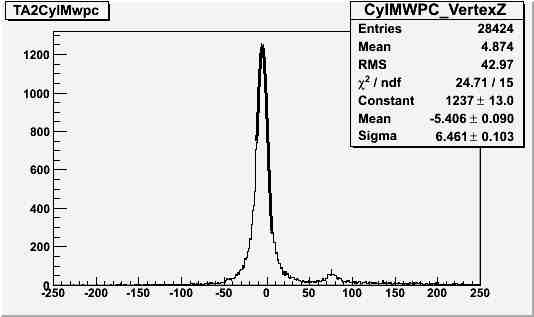
\includegraphics[scale=0.55]{VertexZ_120Sn.png}
\includegraphics[scale=0.55]{VertexZ_124Sn.png}
\caption{Target positioning.}
\label{targetvertex}
\end{center}
\end{figure}

The position of the target have been obtained from a Gaussian fit to the charged particle reaction vertices (Fig. \ref{targetvertex}), the mean of the Gaussian fit have been extracted and the value applied in the analysis as the target position correction.

\indent The obtained value of the position offset with respect to the Crystal Ball have been employed in the analysis code to correct the momenta of the detected particles. The below formulas show how the momentum is calculated for the target located in the centre of the crystal ball (Equation \ref{mom1}) and how the calculation is corrected when the position offset is considered (Equation \ref{mom2}):

\begin{equation}
p = \frac{E_{\meas}}{\sqrt{x^{2}+y^{2}+z^{2}}}(x,y,z)
\label{mom1}
\end{equation}
\begin{equation}
p = \frac{E_{\meas}}{\sqrt{x^{2}+y^{2}+(z-z_{corr})^{2}}}(x,y,z-z_{corr})
\label{mom2}
\end{equation}
where, $E_{\meas}$ is the measured energy of the deposit in the cluster, $x, y, and z$ are the coordinates of the centre of mass of the cluster and $z_{core}$ is the correction due to the target position offset determined with the MWPCs.

\section{Coherent Events}

\indent As described in chapter 2, the $\pi^{0}$ photoproduction can occur in a number of ways, and alongside the coherent process, incoherent and quasi-free reactions also take place. In order to extract the coherent events from the background missing energy analysis has been performed. This technique uses information on incident photon energy from the tagger and $\pi^{0}$ 4-momentum reconstructed from the information recorded in the Crystal Ball.

\indent The pion missing energy is calculated with the following formula:

\begin{equation}
\Delta E_{\pi} = E_{\pi}^{CoM}(E_{\gamma})-E_{\pi}^{CoM}(E_{\gamma_{1}\gamma_{2}})
\end{equation}
where $E_{\pi}^{CoM}(E_{\gamma})=\frac{s+m_{\pi}^{2}-M^{2}}{2\sqrt{s}}$ is the pion energy in the pion-nucleus centre of mass frame of reference. $E_{\gamma}$ in the incident photon energy, $s$ is the invariant mass of the photon-nucleus system and $m_{\pi}$and $M^{2}$ are the masses of pion  and the nucleus respectively. E_{\pi}^{CoM}(E_{\gamma_{1}\gamma_{2}}) is the, Lorentz-transformed to the CoM reference frame, detected pion energy.

\indent Although the pion energy can be simply expressed as the sum of the energies of the two decay photons, considering the angular information of the reaction allows for much better energy resolution, and therefore more accurate calculations \cite{miller}:

\begin{equation}
E_{\pi} = \sqrt{\frac{2m_{\pi}^{2}}{(1-\frac{E_{1}-E_{2}}{E_{1}+E_{2}}^{2})(1-cos\phi)}}
\end{equation}
where, $E_{1}$ and $E_{2}$ are the detected energies of the two decay photons and $\phi$ is the opening angle between them. The Lorentz transformation of the detected pion energy to the CoM frame of reference is calculated with:

\begin{equation}
E_{\pi}^{CoM} = \gamma\Big(E_{\pi}-\frac{E_{\gamma}}{E_{\gamma}+M}\big(E_{1}cos\theta_{1}+E_{2}cos\theta_{2}\big)\Big)
\end{equation}
where, $\theta_{1}$ and $\theta_{2}$ are the polar angles of the two decay photons, $E_{\pi}$ is the detected pion energy.

\indent The condition for the coherent $\pi^{0}$ photoproduction process is that $E_{\pi}^{CoM}(E_{\gamma})$ and $E_{\pi}^{CoM}(E_{\gamma_{1}\gamma_{2}})$ are the same. Background processes however, should return negative values of $\Delta E_{pi}$ since the initial energy is split between other than $\pi^{0}$ particles produced in the reaction, used up to promote the nucleus to an excited state, etc.

\section{Tagging Efficiency}

\indent A tagging efficiency measurements have been performed in order to accurately  determine the beam luminosity which is necessary for the $pi^{0}$ yield normalisation in the cross section measurements. As described in chapter 3, the information about the beam luminosity is obtained from the number of hits in the FP detector. However, when the beam passes through the collimator further photons are removed form it and in order to account for this reduction in the flux a separate measurement with a lower beam intensity is performed.

\indent The tagging efficiency have been measured separately for each target and the results of the measurements are presented in the below figure (Fig. \ref{taggingeff}).

\begin{figure}[H]
\begin{center}
\includegraphics[scale=0.55]{TaggEff_allSn.png}
\caption{Tagging efficiency as a function of channel number for the tin targets.}
\label{taggingeff}
\end{center}
\end{figure}


\section{$\pi^{0}$ detection efficiency}

\indent A Geant4 Monte Carlo simulation has been used to calculate the efficiency of the detector setup.

\indent In order to decrease the time required for the simulation, the minimum number of the generated events have been decided. This number was based on the analysis of the impact on the total error on detection efficiency which depends on the error on generated and reconstructed events. It has been calculated that the error on the reconstructed events in the coherent peak was $\sim1\%$ and the condition of the total error to be at most equal to this value has been imposed. Error calculations yielded that the minimum number of generated events is 10 million.

\indent The $A(\gamma,\pi^{0})A$ events have been generated for the energy range of $135-540MeV$ have been simulated for each target. Then the simulated data were run through the same analysis software as the experimental data. For each energy and $\theta$ bin has been calculated as the the ratio of detected $\pi^{0}'s$ to the total number of $\pi^{0}'s$ generated in that energy and $\theta$ bin.

\indent The dependence of the detection efficiency on the angle is shown in Fig. \ref{detectioneff}. The points at the edges don't follow the polynomial fit because the distribution fluctuates on both sides of the point at the poles and without introducing $\phi$ discrimination it is not possible to improve on this.

\begin{figure}[H]
\begin{center}
\includegraphics[scale=0.55]{DetEff_Eg6.png}
\includegraphics[scale=0.55]{DetEff_Eg7.png}
\includegraphics[scale=0.55]{DetEff_Eg8.png}
\includegraphics[scale=0.55]{DetEff_Eg9.png}
\caption{Dependence of the detection efficiency on energy and $\theta_{\pi^{0}}$ for tin targets.}
\label{detectioneff}
\end{center}
\end{figure}

